\documentclass{article}
\usepackage[UTF8]{ctex}
\usepackage[T1]{fontenc}
\usepackage[utf8]{inputenc}
\usepackage{float}
\usepackage{placeins}
\usepackage{latexsym}
\usepackage{algorithm}
\usepackage{algorithmic}
\usepackage{amsmath}
\usepackage{amsthm}
\title{Homework 1}
\author{PB17000297 罗晏宸}
\date{September 5 2019}

\begin{document}

\maketitle

\section{Exercise 2.1-1}
以图2-2为模型,说明INSERTION-SORT在数组$A=<31,41,59,26,41,58>$上的执行过程。\\
\par
\paragraph{解} 如图\ref{fig:label}

\begin{figure}
\centering
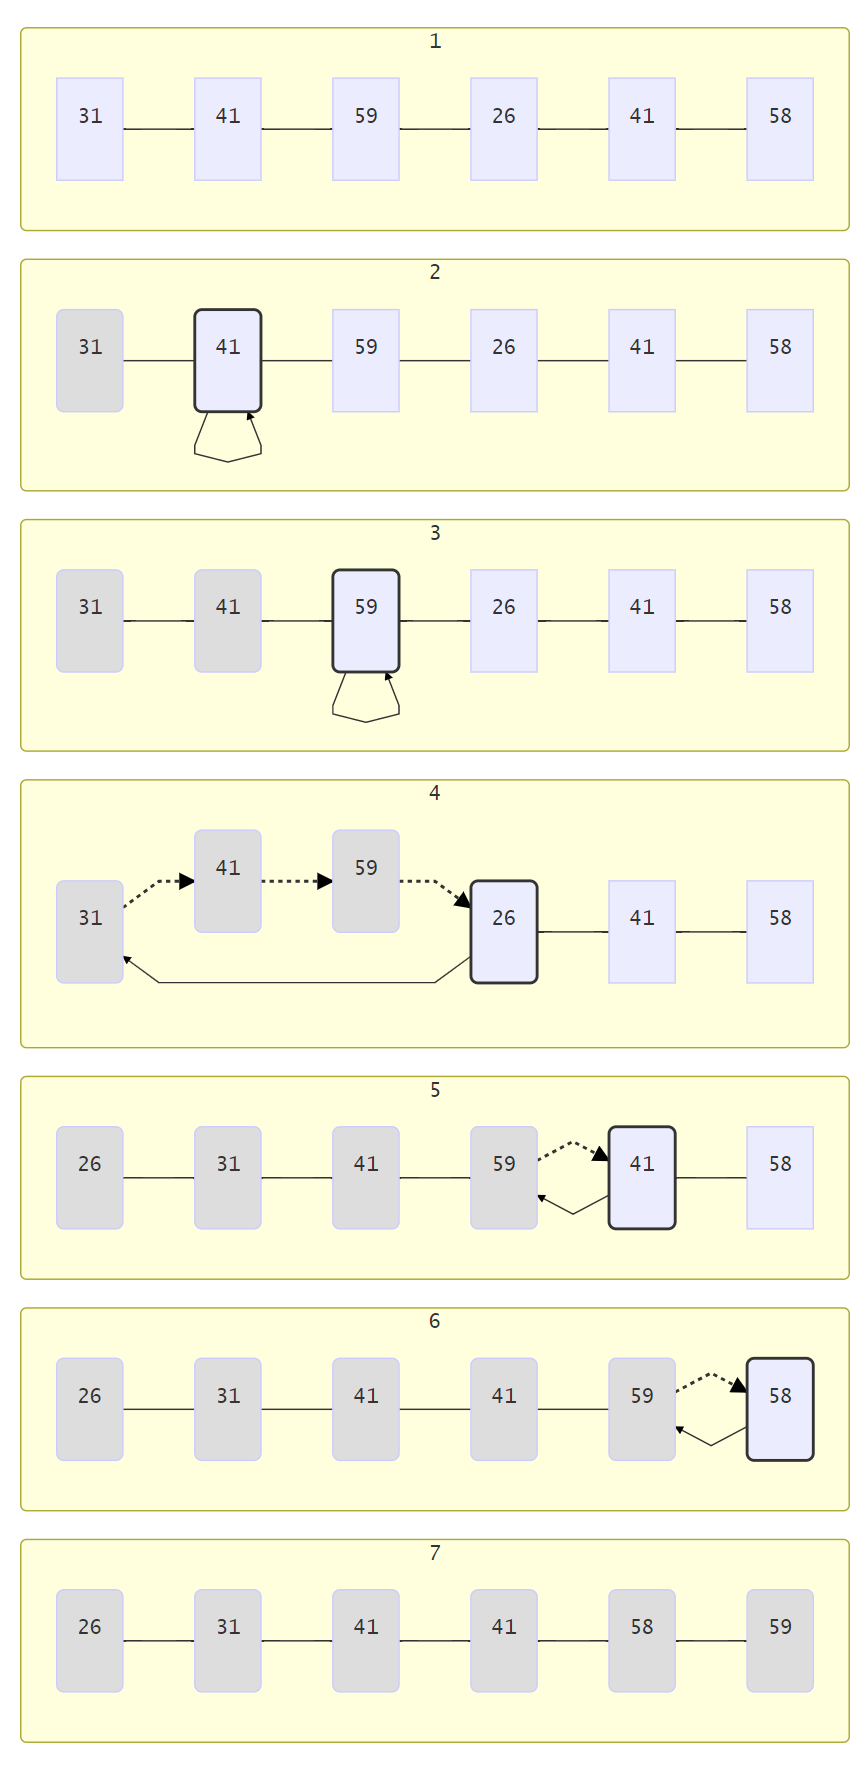
\includegraphics[scale=0.6]{Insertion-sort.png}
\caption{在数组$A=<31,41,59,26,41,58>$上执行INSERTION-SORT的操作。图1~6表示\texttt{for}循环的迭代,每次迭代中,黑框的矩形保存取自A[j]的关键字,它与其左边的矩形中的值作比较,黑色箭头指出它被移到的地方,虚线箭头指出数组值向右移动一个位置。图7表示最终排序好的数组$A=<26,31,41,41,58,59>$。}
\label{fig:label}
\end{figure}

\section{Exercise 2.1-3}
考虑以下\textbf{查找问题}:\par
\textbf{输入}:$n$个数的一个序列$A=<a_1,a_2,\cdots,a_n>$和一个值$v$。\par
\textbf{输出}:下标$i$使得$v=A[i]$或者当$v$不在$A$中出现时,$v$为特殊值$\mathrm{NIL}$。\par
写出\textbf{线性查找}的伪代码,它扫描整个序列来查找$v$。使用一个循环不变式来证明你的算法是正确的,确保你的循环不变式满足三条必要的性质。\\
\par
\paragraph{解}
\FloatBarrier
\begin{algorithm}[h]
\caption{Linear Search}
\label{alg1}
\begin{algorithmic}
\REQUIRE $n \geq 1$
\ENSURE $(A[i] = v)or(i = \textnormal{NIL})$
\STATE $i \gets 1$
\WHILE {$(i \leq n ) and ( a_i \neq v)$}
$i \gets i + 1$
\ENDWHILE
\IF{$i > n$}
\STATE $i \gets \textnormal{NIL}$
\ENDIF
\end{algorithmic}
\end{algorithm}

\par
\textbf{循环不变式}:each $a_j \in A[1..i-1], a_j \neq v$ \par
\textbf{初始化}:在循环的第一次迭代之前,$i = 1, A[1..0] = \emptyset$,循环不变式成立。\par
\textbf{保持}:若在循环的第$m$次迭代之前,循环不变式为真,在第$m+1$次迭代之前,其仍为真,否则说明$a_i = v$即条件$(i \leq n ) and ( a_i \neq v)$不再满足,循环不会进入下一次迭代。 \par
\textbf{终止}:在循环终止时,不变式说明在$A[1..i-1]$不存在与$v$相同的元素,则得到的$i$满足算法的输出要求或$i > n$输出相应的结果\text{NIL}。

\section{Exercise 2.2-3}
再次考虑线性查找问题(参见练习2.1-3)。假定要查找的元素等可能地为数组中的任意元素,平均需要检查输入序列的多少元素?最坏情况又如何呢?用$\Theta$记号给出线性查找的平均情况和最坏情况运行时间。证明你的答案。\\
\par
\paragraph{解}
设$X(i)$为要查找的元素$v$为$a_i$时检查的元素数,$P(i)$为要查找的元素$v$为$a_i$的概率,则$X(i)=i,P(i)=\displaystyle \frac{1}{n},\quad i=1,\cdots,n$,有
\begin{align*}
    \mathrm{E}[X]&=\sum_{i=1}^n{X(i)P(i)} \\
    &=\sum_{i=1}^n{i \cdot \frac{1}{n}} \\
    &=\frac{n(n+1)}{2}\cdot\frac{1}{n} \\
    &=\frac{n+1}{2}
\end{align*}
即平均需要检查输入序列的元素数为$\displaystyle \frac{n+1}{2}$。\par
在最坏的情况下,每次都需要检查输入序列中的所有元素,即$X_{worst}(i) \equiv n$,有
\begin{align*}
    \mathrm{E}_{worst}[X]&=\sum_{i=1}^n{X_{worst}(i)P(i)} \\
    &=\sum_{i=1}^n{n \cdot \frac{1}{n}} \\
    &=n
\end{align*}
即最坏情况下,平均需要检查输入序列的元素数为$n$。\par
在平均情况下,线性查找的运行时间为
\begin{align*}
    T(n)&=\mathrm{E}[X]+2 \\
    &=\frac{n+1}{2} +2 \\
    &=\Theta(n)
\end{align*} \par
\begin{proof}
    事实上,当$n \geq 5$时,对于常数$1$和$2$,恒有
    1 \cdot (\frac{n+1}{2}+2)=\frac{n+1}{2} + 2 \leq n \leq n+5= 2 \cdot (\frac{n+1}{2}+2)
\end{proof} \par
在最坏情况下,线性查找的运行时间为
\begin{align*}
    T(n)&=\mathrm{E}_{worst}[X]+2 \\
    &=n+2 \\
    &=\Theta(n)
\end{align*} \par
\begin{proof}
    事实上,当$n \geq 2$时,对于常数$\displaystyle \frac{1}{2}$和$1$,恒有
    0.5\cdot(n+2)=\frac{1}{2}\cdot n + 1 \leq n \leq n+2= 1\cdot(n+2)
\end{proof} \par
\end{document}